\section{Theoretical Analysis}
\label{sec:analysis}

In this section, the circuit shown in \textbf{Figure~\ref{fig:circuit_t1}} is analysed
theoretically using two methods: the mesh analysis and the nodal analysis.\par


\subsection{Nodal Analysis} 
For the nodal analysis we apply the Kirchhoff Current Law (KCL) to the nodes that are not conected to voltage sources (equations \ref{eq:n3} to \ref{eq:n7}). We obtain 2 more equations from the potencial difference at the terminals of the voltage sources (equations \ref{eq:n8} and \ref{eq:n9}). As was stated before, {\it node 0} is the ground node and therefore the voltage at this node is 0V (equation \ref{eq:n1}). For the simulation analysis it was necessesary to add another "fictional" voltage source that provides 0 volts to the circuit, between node 7 and resistor 6. This "fictional" voltage source was also considered in the Theoretical Analysis, as it has no real effect on the circuit. It was needed to define in the ngspice code the current on which the current-controlled voltage source depends on. This yields equation number \ref{eq:n2}. Now we have 9 equations for 9 unkown variables - voltage {\it$V_{0}$}  to {\it$V_{8}$}. The schematics correponding to this approach can be seen in \textbf{Figure~\ref{fig:circuit_t2}} Using Octave, we determine the values of every node voltage of the circuit. \par

\begin{figure}[h] \centering
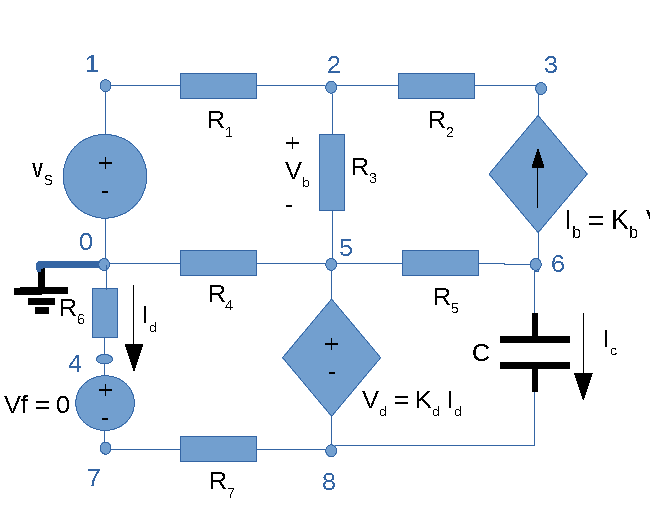
\includegraphics[width=0.9\linewidth]{diagram_t2.pdf}
\caption{Diagram of the circuit considered for the computations}
\label{fig:diagram_t2}
\end{figure}

\begin {equation}
	V_0 = 0
	\label{eq:n1}
\end{equation}
\begin {equation}
	V_8 = V_7
	\label{eq:n2}
\end{equation}
\begin {equation}
	\frac{V_1-V_2}{R_1} + \frac{V_0 - V_8}{R_6} + \frac{V_0 - V_4}{R_4} = 0
	\label{eq:n3}
\end{equation}
\begin {equation}
	\frac{V_2-V_4}{R_3} + \frac{V_2-V_3}{R_2} + \frac{V_2-V_1}{R_1} = 0
	\label{eq:n4}
\end{equation}
\begin {equation}
	- K_b(V_2-V_4) + \frac{V_3-V_2}{R_2} = 0
	\label{eq:n5}
\end{equation}
\begin {equation}
	\frac{V_5-V_4}{R_5} + K_b(V_2-V_4) - Id = 0
	\label{eq:n6}
\end{equation}
\begin {equation}
	\frac{V_7-V_6}{R_7} + \frac{V_7 - V_0}{R_6} = 0
	\label{eq:n7}
\end{equation}
\begin {equation}
	V_1 - V_0 = V_a
	\label{eq:n8}
\end{equation}
\begin {equation}
	V_4 - V_6 = K_c  \frac{V_0 - V_7}{R_6}
	\label{eq:n9}
\end{equation}


In \textbf{Table~\ref{tab:theoretical}} the values for the branch currents and the node voltages obtained from the Octave script for both methods are presented. Here, the node voltages in the mesh method were computed from the respective currents, which were determined as described in the previous subsection.
 \pagebreak 
\begin{table}[h]
  \centering
  \begin{tabular}{|l|r|}
    \hline    
    {\bf Name} & {\bf Node method}\\ \hline
    V0 & 0\\ \hline
V1 &  5.054818641360000\\ \hline
V2 &  4.793704691824189\\ \hline
V3 &  4.258197784082119\\ \hline
V4 & -1.934225550007436\\ \hline
V5 &  4.831047093349573\\ \hline
V6 &  5.668298372306746\\ \hline
V7 & -1.934225550007436\\ \hline
V8 & -2.905231322705667\\ \hline
Ir1 &   -2.536487650531725e-01\\ \hline
Ir2 &   -2.658975828505401e-01\\ \hline
Ir3 &    1.224881779736725e-02\\ \hline
Ir4 &  1.205310280142027\\ \hline
Ir5 &    2.658975828505403e-01\\ \hline
Ir6 &   -9.516615150888543e-01\\ \hline
Ir7 &   -9.516615150888547e-01\\ \hline
Gbn &    2.658975828505403e-01\\ \hline

  \end{tabular}
  \caption{A variable preceded by @ is of type {\em current}
    and expressed in milliampere (mA); other variables are of type {\it voltage} and expressed in
    Volt (V).}
  \label{tab:theoretical}
\end{table}


As can be seen, the values obtained via the mesh and the node analysis are the same, which suggests that for this simple circuit, the methods are equally precise, as expected.

\subsection{Equeivalent resistor form capacitor's prespective} 




In \textbf{Table~\ref{tab:theoretical}} the values for the branch currents and the node voltages obtained from the Octave script for both methods are presented. Here, the node voltages in the mesh method were computed from the respective currents, which were determined as described in the previous subsection.
 \pagebreak 
\begin{table}[h]
  \centering
  \begin{tabular}{|l|r|}
    \hline    
    {\bf Name} & {\bf Values for aux circuit}\\ \hline
    @Gb & 0.00000000000\\ \hline
@r1 & 0\\ \hline
@r2 & 0\\ \hline
@r3 & 0\\ \hline
@r4 & 0\\ \hline
@r5 &   -2.828260531660058e-03\\ \hline
@r6 & 0\\ \hline
@r7 & 0\\ \hline
v(1) & 0.00000000000\\ \hline
v(2) & 0.00000000000\\ \hline
v(3) & 0.00000000000\\ \hline
v(4) & 0.00000000000\\ \hline
v(5) & 0.00000000000\\ \hline
v(6) & 8.83130397945\\ \hline
v(7) & 0.00000000000\\ \hline
v(8) & 0.00000000000\\ \hline
Ix & -0.00282826053\\ \hline
Vx & 8.83130397945\\ \hline
$Req_{}$ & -3.122521e+03\\ \hline
$\tau$ & -3.181599e-03\\ \hline
  \end{tabular}
  \caption{A variable preceded by @ is of type {\em current}
    and expressed in milliampere (mA); other variables are of type {\it voltage} and expressed in
    Volt (V).}
  \label{tab:equivalent resistor}
\end{table}


As can be seen, the values obtained via the mesh and the node analysis are the same, which suggests that for this simple circuit, the methods are equally precise, as expected.





